%%%%%%%%%%%%%%%%%%%%%%%%%%%%%%%%%%%%%%%%%
% University/School Laboratory Report
% LaTeX Template
% Version 3.1 (25/3/14)
%
% This template has been downloaded from:
% http://www.LaTeXTemplates.com
%
% Original author:
% Linux and Unix Users Group at Virginia Tech Wiki
% (https://vtluug.org/wiki/Example_LaTeX_chem_lab_report)
%
% License:
% CC BY-NC-SA 3.0 (http://creativecommons.org/licenses/by-nc-sa/3.0/)
%
%%%%%%%%%%%%%%%%%%%%%%%%%%%%%%%%%%%%%%%%%

%----------------------------------------------------------------------------------------
%	PACKAGES AND DOCUMENT CONFIGURATIONS
%----------------------------------------------------------------------------------------

\documentclass[a4paper,10pt]{article}

\usepackage{graphicx} % Required for the inclusion of images
\usepackage{natbib} % Required to change bibliography style to APA
\usepackage{amsmath} % Required for some math elements
\usepackage{hyperref} % HTTP links
\usepackage[utf8]{inputenc}
\usepackage[T1]{fontenc} % Accented letters
\usepackage{hhline}
\usepackage{pgfplots}
\usepackage{tabularx}
\usepackage[italian]{babel}
\usepackage[title]{appendix}
\pgfplotsset{width=7cm,compat=1.8}

\setlength\parindent{0pt} % Removes all indentation from paragraphs

%\renewcommand{\labelenumi}{\alph{enumi}.} % Make numbering in the enumerate environment by letter rather than number (e.g. section 6)

%----------------------------------------------------------------------------------------
%	DOCUMENT INFORMATION
%----------------------------------------------------------------------------------------

\title{Schema Matching con Algoritmo di Similarity Flooding \\ Progetto di Ingegneria Informatica 2019/2020\\
\large (Draft version 2)} % Title

\author{Stefan \textsc{Djokovic} \\
	\texttt{stefan.djokovic@mail.polimi.it}
	\and Kien Tuong \textsc{Truong} \\
	\texttt{kientuong.truong@mail.polimi.it}} % Author name

\date{\today} % Date for the report

\begin{document}

\maketitle % Insert the title, author and date

\begin{center}
\begin{tabular}{l r}
Referenti: & Prof. Letizia Tanca\\ % Partner names
& Fabio Azzalini PhD Candidate
\end{tabular}
\end{center}

% If you wish to include an abstract, uncomment the lines below
% \begin{abstract}
% Abstract text
% \end{abstract}

%----------------------------------------------------------------------------------------
%	SECTION 1
%----------------------------------------------------------------------------------------

\section{Introduzione}

Da decenni il problema di integrare dati provenienti da fonti differenti e con formati differenti è stato centro dell’attenzione di molte pubblicazioni scientifiche. La necessità di ottenere una visione di insieme a partire da schemi eterogenei è essenzialmente guidata dal bisogno che ricercatori e aziende hanno nel raggruppare una vasta quantità di dati, al fine di utilizzare quest’ultimi in ambito accademico o commerciale. Questo ambito è comunemente indicato con il termine “Data Integration”.\\

In particolare, il processo di unificare gli schemi di due database è chiamato “Schema Matching”. Più formalmente lo schema matching consiste nel trovare quali oggetti, provenienti da schemi differenti, sono correlati semanticamente.\\

La problematica principale, che è anche il motivo per cui molta ricerca viene effettuata in questo ambito, è che lo schema matching è un processo non facilmente automatizzabile in quanto dipende dalla capacità di comprendere il legame semantico esistente tra più elementi, capacità sicuramente non banale da esprimere in modo algoritmico.\\

È in questo contesto che si pone il lavoro di Sergey Melnik, Hector Garcia-Molina ed Erhard Rahm, riassunto nel paper “Similarity Flooding: A Versatile Graph Matching Algorithm
and its Application to Schema Matching” \cite{sfpaper}. L’obiettivo preposto nel paper è quello di creare un algoritmo generale (in contrasto con algoritmi più domain-specific) per effettuare euristicamente schema matching e misurarne l’utilità mediante il lavoro in meno che un umano deve compiere rispetto allo schema matching interamente manuale.


\section{Termini di Riferimento}

Il progetto è svolto nel contesto del corso “Progetto di Ingegneria Informatica” del corso di studi di Ingegneria Informatica al Politecnico di Milano, il cui titolare è il prof. Fabio Salice.\\

I referenti del progetto sono la prof.ssa. Letizia Tanca e Fabio Azzalini\\

I membri del team di sviluppo sono Stefan Djokovic (886860) e Kien Tuong Truong (887907).\\

Una discussione iniziale con il referente del progetto è risultata nella scelta di Python 3 come linguaggio di sviluppo, sia per la semplicità e per la rapidità di sviluppo, ma anche per la disponibilità della libreria NetworkX per comoda gestione dei grafi.\\

L’implementazione finale può essere trovata sulla repository di Github:\\
\url{https://github.com/kientuong114/SimilarityFlooding}

%----------------------------------------------------------------------------------------
%	SECTION 3
%----------------------------------------------------------------------------------------

\section{Descrizione dell'Algoritmo}
\label{descript_alg}

L’algoritmo, nella sua forma più astratta, si basa su un principio di similitudine topografica tra grafi. L’intuizione è la seguente: se è noto che un nodo di un grafo ed un nodo di un altro grafo sono simili tra di loro (per una qualche definizione di similitudine) allora si può propagare la similarità ai loro nodi adiacenti.\\
Più formalmente, siano $G_1 = (V_1, E_1)$ e $G2 = (V_2, E_2) $ due grafi e sia \\ $S: V1\times V2 \to [0, 1]$ una funzione di similitudine: l’idea è quella di generare un unico grafo a partire da G1 e G2 in cui ogni nodo rappresenta la similitudine tra una coppia di nodi, uno appartenente a G1 e l’altro appartenente a G2.\\

Si va poi a fissare una similitudine iniziale $S_0$ applicando $S$ su ogni coppia di nodi e iterativamente sfruttare la similitudine iniziale di ogni nodo per computare le nuove similitudini dei nodi adiacenti $S_1$, mediante una funzione delta di propagazione. Questo processo viene iterato fino ad una certa condizione di terminazione.\\

Alla fine del processo si estraggono euristicamente i risultati che hanno una similitudine maggiore.\\

A seguito descriviamo più in profondità l’algoritmo nella sua applicazione al matching di schemi di database: uno schema (SQL, XML,...) viene convertito nella sua rappresentazione a grafo parsando la sua rappresentazione testuale e costruendo il grafo secondo le linee guida definite. Vi è da sottolineare come il paper non abbia una particolare preferenza rispetto al modo con cui lo schema viene convertito in grafo. Ai fini del progetto si è scelto di rimanere fedeli alla metodologia descritta da Melnik in \citep{generic_model_man}.\\

A partire da due grafi si computa la similitudine iniziale, descritta nel paper come Initial Mapping. La funzione di similitudine iniziale scelta si basa sulla distanza di Levenshtein tra stringhe, per cui si è utilizzata la libreria FuzzyWuzzy per Python. Questo è l’unico passo dell’algoritmo che si basa su proprietà non topologiche del grafo.\\

Successivamente vengono creati due grafi di supporto alla computazione principale dell’algoritmo: il Pairwise Connectivity Graph (PCG) e l’Induced Propagation Graph (IPG), costruito a partire dal PCG.\\

Il Pairwise Connectivity Graph è un grafo che possiede come nodi coppie del tipo $(x,y)$ con $x\in E_{G_1}$ e $y\in E_{G_2}$ (Cioè $x$ è un nodo di $G_1$ e $y$ è un nodo di $G_2$) e per cui vale che $((x,y), p, (x', y')) \in E_{IPG} \Leftrightarrow (x, p, x') \in E_{G_1} \wedge (y, p, y') \in E_{G_2}$, in altre parole due nodi dell'IPG sono collegati tra loro da un arco con label $p$ se e solo se le coppie di nodi coinvolte $(x, x')$ e $(y, y')$ appartengono rispettivamente a $G_1$ e $G_2$ e sono tra di loro connesse da un arco con label $p$.\\

\begin{figure}
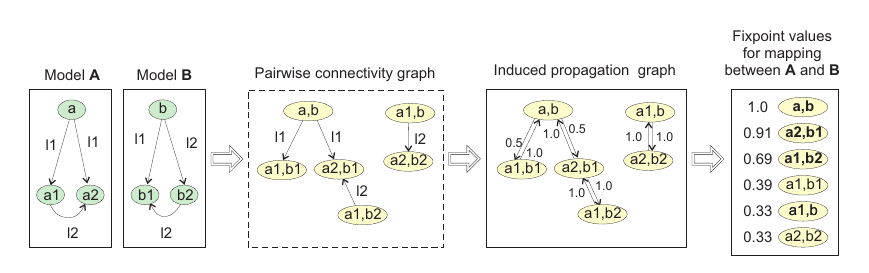
\includegraphics[scale=0.4]{sf.png}
\caption{Esempio di aplicazione dell'algoritmo su un semplice grafo}
\label{sf1}
\end{figure}

Per un'esempio grafico si veda l'immagine \ref{sf1}.\\

Da questo PCG viene generato l'Induced Propagation Graph, cioè il grafo che possiede tutti gli stessi nodi del PCG e che, per ciascuna coppia di nodi del PCG collegata da un arco, presenta una coppia di archi, uno per ciascuna direzione, a cui è associato un determinato valore, che rappresenta il coefficiente di propagazione da un nodo all'altro, nella direzione dell'arco.\\

Tale coefficiente di propagazione uscente da ciascun nodo dell'IPG è calcolato come il reciproco del numero di archi (uscenti o entranti) dal corrispondente nodo del PCG che condividono lo stesso label. In pratica, se un nodo del PCG possiede 4 archi (uscenti o entranti) con un certo label $p$, allora il suo contributo nell'IPG ai nodi adiacenti sarà pari a $1/4$.\\

L’IPG è il grafo su cui viene computato l’algoritmo di flooding vero e proprio (chiamato nel paper Fixpoint Computation). Ogni nodo riceve il contributo di tutti i nodi ad esso adiacenti, mediante una funzione (Fixpoint Formula) che dipende dai coefficienti di propagazione associata agli archi entranti nel nodo. Quando la similitudine per ciascun nodo è stata computata, ogni valore è normalizzato rispetto al massimo valore di similitudine presente nel grafo. Ciò fa in modo che i nodi in assoluto più simili possiedano una similitudine di 1.\\

L’algoritmo viene iterato sull’IPG fino a quando non si arriva ad una condizione di terminazione, che può essere la stabilità dell’algoritmo entro una certa variazione epsilon tra un passo ed il successivo (configurabile), oppure un numero fissato di passi.\\

Dai risultati della computazione sull’IPG si estraggono i migliori match, mediante uno stadio che il paper definisce come "filter". L'algoritmo di filter deve implementare una qualche euristica per selezionare i match migliori partendo dai risultati della fixpoint computation. L'algoritmo da noi implementato per questo step si basa sul problema conosciuto nella letteratura scientifica come il problema del matrimonio stabile (Stable marriage problem).\\

Si noti che, sebbene qui sia stato descritto l'algoritmo più nello specifico nell'ambito dello Schema Matching, esso è estendibile a qualsiasi applicazione rappresentabile con grafi e dai quali è possibile estrarre una certo valore di similarità tra nodi di grafi differenti. \\

%----------------------------------------------------------------------------------------
%	SECTION 4
%----------------------------------------------------------------------------------------

\section{Timeline del Progetto}

Il primo passo effettuato è stato quello di ricercare più approfonditamente il paper fornito, che ha portato alla scoperta di una versione estesa del paper \cite{sfpaper_ext} e anche alla dissertazione di PhD di uno degli autori \cite{generic_model_man}.\\

La ricerca ha fornito spunti di approfondimento su alcuni passaggi trattati rapidamente nel paper, in particolare sulla trasformazione da schema di database a grafo, che è stato il primo passo nello sviluppo del progetto.
Dopo aver sviluppato i primi parser di schemi SQL e XML si è sviluppato ogni passo dell’algoritmo separatamente ed indipendentemente.\\

Il progetto è stato sviluppato mantenendo contatti con i referenti del progetto, con cui sono stati condivisi dubbi a livello tecnico e che hanno fornito vari casi di test su cui sperimentare l’implementazione.\\

Il progetto finale comprende vari parser per i formati SQL schema, XML e XDR, i moduli che implementano l’algoritmo ed alcuni casi di test, che hanno guidato lo sviluppo.\\

%----------------------------------------------------------------------------------------
%	SECTION 5
%----------------------------------------------------------------------------------------

\section{Scelte Progettuali}
\label{Scelte Progettuali}

Il paper non pone alcuna preferenza riguardo al tipo di schema di input. Come scelta progettuale si sono sviluppati 3 moduli di parsing: uno per schemi SQL, rappresentati mediante DDL, schemi XML e XDR. La scelta è stata guidata dalla popolarità di tali schemi (SQL e XML) oppure perchè era il formato principale degli schemi di test forniti (XDR).\\

Una divergenza rispetto al paper, guidata da alcune intuizioni apparse durante lo sviluppo del progetto, è stata nella generazione del grafo iniziale: il paper presenta un modello che rappresenta ogni entità come un nodo caratterizzato da un nominativo univoco detto OID (della forma "\&num", dove num è un numero naturale). Per indicare il nome reale di tale entità, tale nodo viene collegato ad un altro nodo rappresentante il nome, da un arco che rappresenta la relazione “nome di”. \\

È stato osservato che questo dettaglio va ad influenzare fortemente i risultati dell’algoritmo. La motivazione è intuibile mediante il fatto che la similitudine iniziale data dall’Initial Mapping è una proprietà del contenuto del nodo (si noti che a questo fine gli OID non erano considerati, in quanto altrimenti ogni OID sarebbe risultato molto simile ad ogni altro OID) mentre il resto dell’algoritmo si basa su proprietà strutturali del grafo. Questo fa in modo che la similitudine iniziale tra due nodi, in alcuni casi anche molto alta, venisse “dispersa” in quanto i nodi con i nomi non erano collegati direttamente al resto del grafo, ma solamente mediante i nodi di OID.\\

La mancanza di queste considerazioni nelle documentazioni originali e l'assenza degli OID nella maggior parte delle rappresentazioni dei grafi ci ha portato a sviluppare entrambe le soluzioni, offrendo entrambe le opzioni alla generazione del grafo: a partire da un grafo con gli OID si può effettuare l’algoritmo direttamente su tale grafo, oppure si può effettuare un’ulteriore trasformazione di compressione sul grafo, in modo da rimuovere gli OID. Un confronto tra i risultati su grafi compressi e non compressi è presente nella sezione 7 di questo report.\\

Infine, nel contesto del paper sono state presentate varie alternative riguardo alla scelta della Fixpoint Formula. Per testare tutte le varie possibilità si è scelto di implementare tutte e 4 le formule presentate in \citep{sfpaper_ext}, lasciando la possibilità di cambiare la funzione da utilizzare.


%----------------------------------------------------------------------------------------
%	SECTION 6
%----------------------------------------------------------------------------------------

\section{Moduli del progetto}

Il progetto è composto da 4 moduli principali, organizzati in diverse sottocartelle pubblicate sulla repository su GitHub per permettere la facile modifica dei singoli:
\begin{enumerate}
	\item \textbf{parse}: contiene parser SQL DDL, XDR e XML usati per testare l'algoritmo e sono esempio di conversione da file a grafo NetworkX
	\item \textbf{initialmap}: contiene un algoritmo di attraversamento dei nodi dei due grafi per generare l'initialMap dei due, ossia il valore di similitudine al quale vengono inizializzati i nodi corrispondenti
	\item \textbf{sf}: contiene l'algoritmo di generazione del PCG e dell'IPG (spiegati nel paragrafo \ref{descript_alg}), la loro inizializzazione, e l'algoritmo di Similarity Flooding, con le 4 formule Fixpoint presentate nel paper originali. 
	\item \textbf{filter}: contiene un filtro del risultato ottenuto dal Similarity Flooding basato sull'algoritmo di Stable Marriage.
\end{enumerate}
Questi permettono di poter eseguire l'intero processo di schema matching, e sono sufficientemente documentati e robusti da permettere la facile integrazione con altri progetti. L'utilizzo di Python e NetworkX, in particolare, facilitano questo processo, essendo il primo un linguaggio molto usato in Data Science, ed essendo il secondo una libreria molto usata per la generazione e studio di grafi su Python.\\

La repository del progetto contiene inoltre la cartella \textbf{test} con degli esempi di funzioni per permettere la generazione dei risultati e un algoritmo che automatizza la valutazione dell'output (e con il quale sono stati estratti i risultati della sezione 7 di questo report). È presente infine la cartella \textbf{utils} che contiene varie funzioni utilizzate in diversi punti del progetto.

%----------------------------------------------------------------------------------------
%	SECTION 7
%----------------------------------------------------------------------------------------

\section{Risultati}

Riportiamo alcuni risultati ottenuti mediante il matching di alcuni schemi fornitici, assieme ai risultati attesi corredati agli schemi.\\

Per i test si userà la seguente terminologia:
\begin{enumerate}
	\item \textbf{True Positive}: L'algoritmo ha determinato che un elemento ha un match ed effettivamente possiede quel match.
	\item \textbf{True Negative}: L'algoritmo ha determinato che un elemento non ha un match ed effettivamente non possiede match.
	\item \textbf{False Positive}: L'algoritmo ha determinato che un elemento ha un match ma in realtà questo non è esistente
	\item \textbf{False Negative}: L'algoritmo ha determinato che un elemento non ha un match ma in realtà questo è esistente.
\end{enumerate}

Inoltre si distinguono i casi in cui il grafo è stato compresso (Compressed), cioè i suoi OID sono stati sostituiti dal nome vero dell'oggetto (si veda la sezione \ref{Scelte Progettuali}), oppure in cui il grafo non è stato compresso (Non Compressed).

\newpage

\subsection{Test Case 1: Apertum + CIDXPOSCHEMA (XDR)}

Il seguente test case è preso dai dataset di benchmark della Universitat Leipzig (Reperibili a \url{https://dbs.uni-leipzig.de/en/bdschemamatching}).\\

A seguito due tabelle riassuntive dei risultati ottenuti al variare della Fixpoint Formula e della compressione o meno del grafo\\

\textbf{Grafo non compresso}

\begin{center}
\begin{tabular}{| l | c | c | c | c |}
	\hline
	\textbf{Fixpoint Formula} & Incremental & A & B & C\\
	\hhline{|=|=|=|=|=|}
	\textbf{True Positives} & 1 & 9 & 9 & 9\\
	\hline
	\textbf{True Negatives} & 49 & 51 & 51 & 51\\
	\hline
	\textbf{False Positives} & 39 & 31 & 31 & 31\\
	\hline
	\textbf{False Negatives} & 13 & 11 & 11 & 11\\
	\hline
	\textbf{Accuracy} & 49.02\% & 58.82\% & 58.82\% & 58.82\%\\
	\hline
	\textbf{Precision} & 2.5\% & 22.5\% & 22.5\% & 22.5\%\\
	\hline
	\textbf{Recall} & 7.14\% & 45.00\% & 45.00\% & 45.00\%\\
	\hline
\end{tabular}
\end{center}
\vspace{4mm}

\textbf{Grafo compresso}

\begin{center}
\begin{tabular}{| l | c | c | c | c |}
	\hline
	\textbf{Fixpoint Formula} & Incremental & A & B & C\\
	\hhline{|=|=|=|=|=|}
	\textbf{True Positives} & 1 & 7 & 2 & 7\\
	\hline
	\textbf{True Negatives} & 47 & 51 & 47 & 50\\
	\hline
	\textbf{False Positives} & 39 & 33 & 38 & 33\\
	\hline
	\textbf{False Negatives} & 15 & 11 & 15 & 12\\
	\hline
	\textbf{Accuracy} & 47.06\% & 56.86\% & 48.04\% & 55.88\%\\
	\hline
	\textbf{Precision} & 2.5\% & 17.5\% & 5.0\% & 17.5\%\\
	\hline
	\textbf{Recall} & 6.25\% & 38.89\% & 11.76\% & 36.84\%\\
	\hline
\end{tabular}
\end{center}
\vspace{2mm}

\begin{center}
\begin{tikzpicture}
\begin{axis}
[
	width=\textwidth,
	height=0.5\textwidth,
    ybar=5.5mm,
    ymax = 25,
    ymin = 0,
    enlarge x limits=0.35,
    legend style={at={(0.5,-0.2)},
      anchor=north,legend columns=-1},
    ylabel={\% Precision},
    symbolic x coords={No Compression, Compression},
    xtick=data,
    nodes near coords,
    nodes near coords align={vertical},
]
\addplot coordinates {(No Compression, 2.5) (Compression, 2.5)};
\addplot coordinates {(No Compression, 22.5) (Compression, 17.5)};
\addplot coordinates {(No Compression, 22.5) (Compression, 5.0)};
\addplot coordinates {(No Compression, 22.5) (Compression, 17.5)};
\legend{Incremental, A, B, C}
\end{axis}
\end{tikzpicture}
\end{center}

\begin{center}
\begin{tikzpicture}
\begin{axis}
[
	width=\textwidth,
	height=0.5\textwidth,
    ybar=5.5mm,
    ymax = 55,
    ymin = 0,
    enlarge x limits=0.35,
    legend style={at={(0.5,-0.2)},
      anchor=north,legend columns=-1},
    ylabel={\% Recall},
    symbolic x coords={No Compression, Compression},
    xtick=data,
    nodes near coords,
    nodes near coords align={vertical},
]
\addplot coordinates {(No Compression, 7.14) (Compression, 6.25)};
\addplot coordinates {(No Compression, 45) (Compression, 38.89)};
\addplot coordinates {(No Compression, 45) (Compression, 11.76)};
\addplot coordinates {(No Compression, 45) (Compression, 36.84)};
\legend{Incremental, A, B, C}
\end{axis}
\end{tikzpicture}
\end{center}

\begin{center}
\begin{tikzpicture}
\begin{axis}
[
	width=\textwidth,
	height=0.5\textwidth,
    ybar=5.5mm,
    ymax = 65,
    ymin = 40,
    enlarge x limits=0.35,
    legend style={at={(0.5,-0.2)},
      anchor=north,legend columns=-1},
    ylabel={\% Accuracy},
    symbolic x coords={No Compression, Compression},
    xtick=data,
    nodes near coords,
    nodes near coords align={vertical},
]
\addplot coordinates {(No Compression, 49.02) (Compression, 47.06)};
\addplot coordinates {(No Compression, 58.82) (Compression, 56.86)};
\addplot coordinates {(No Compression, 58.82) (Compression, 48.04)};
\addplot coordinates {(No Compression, 58.82) (Compression, 55.88)};
\legend{Incremental, A, B, C}
\end{axis}
\end{tikzpicture}
\end{center}

Si può osservare come, tendenzialmente, la formula A dia dei risultati migliori in generale, probabilmente dati dall'ampio numero di veri negativi (cioè casi in cui l'algoritmo ha determinato correttamente l'assenza di un corrispettivo nell'altro grafo). Nonostante tale numero possa risultare meno utile del numero di veri positivi, i risultati possono essere comunque usati per sfoltire il numero di campi su cui effettuare matching manuale. Questo dato è particolarmente accentuato in questo test case, dove uno degli schemi è significativamente più piccolo dell'altro (80 linee di CIDXPOSCHEMA.xdr contro 335 linee di Apertum.xdr).\\

Si veda la tabella \ref{results1} per le similitudini selezionate dall’algoritmo nel caso migliore, cioè grafo non compresso e fixpoint formula A.

\begin{table}
\noindent\makebox[\textwidth]{%
\begin{tabular}{| c | c | c |}
	\hline
	\textbf{Apertum} & \textbf{CIDXPOSCHEMA} & \textbf{Risultato}\\
	\hhline{|=|=|=|}
PO.POHeader & Order.POHead.OrderDetails &				True Positive \\
\hline
PO.POHeader.poDate & Order.POHead.TermsOfPayment &                      False Positive\\
\hline
PO.POHeader.poNumber & Order.POHead.TermsOfDelivery &                   False Positive\\
\hline
PO & Order &                                                            True Positive\\
\hline
PO.Contact & Order.Buyer.Contact &                                      True Positive\\
\hline
PO.Contact.contactName & Order.Buyer.Contact.LastName &                 True Positive\\
\hline
PO.Contact.contactFunctionCode & Order.Buyer.Contact.JobTitle &         False Positive\\
\hline
PO.Contact.contactEmail & Order.Buyer.Contact.EMail &                   True Positive\\
\hline
PO.Contact.contactPhone & Order.Buyer.Contact.Phone &                   True Positive\\
\hline
PO.POShipTo & Order.OrderTotal.TotalAmount &                            False Positive\\
\hline
PO.POShipTo.entityidentifier & Order.POLine.Quantity.UnitOfMeasure &    False Positive\\
\hline
PO.POShipTo.city & Order.POHead.Currency &                              False Positive\\
\hline
PO.POShipTo.attn & Order.POLine.Product.EAN &                           False Positive\\
\hline
PO.POShipTo.country & Order.InvoiceTo.Contact &                         False Positive\\
\hline
PO.POShipTo.stateProvince & Order.OrderTotal.NumberOfLines &            False Positive\\
\hline
PO.POShipTo.street4 & Order.POLine.Amount.Amount\_ExclVAT &              False Positive\\
\hline
PO.POShipTo.street3 & Order.POLine.Amount.VAT\_Rate &                    False Positive\\
\hline
PO.POShipTo.street2 & Order.POLine.Product.SupplierPartDesc &           False Positive\\
\hline
PO.POShipTo.street1 & Order.POHead &                                    False Positive\\
\hline
PO.POShipTo.postalCode & Order.DeliverTo.Contact &                      False Positive\\
\hline
PO.POBillTo & Order.POLine &                                            False Positive\\
\hline
PO.POBillTo.entityidentifier & Order.POLine.Quantity.PackSize &         False Positive\\
\hline
PO.POBillTo.city & Order.Buyer.Address.City &                           False Positive\\
\hline
PO.POBillTo.attn & Order.InvoiceTo.VAT\_RegistrationNo &                 False Positive\\
\hline
PO.POBillTo.country & Order.POLine.Amount &                             False Positive\\
\hline
PO.POBillTo.stateProvince & Order.InvoiceTo.SupplierReferenceNo &       False Positive\\
\hline
PO.POBillTo.street4 & Order.InvoiceTo.Address &                         False Positive\\
\hline
PO.POBillTo.street3 & Order.Buyer.Address.Street &                      False Positive\\
\hline
PO.POBillTo.street2 & Order.InvoiceTo.BuyerReferenceNo &                False Positive\\
\hline
PO.POBillTo.street1 & Order.POLine.RequestedDeliveryDate &              False Positive\\
\hline
PO.POBillTo.postalCode & Order.Buyer.Address.PostCode &                 False Positive\\
\hline
PO.POLines & Order.Buyer.Address &                                      False Positive\\
\hline
PO.POLines.startAt & Order.POLine.Amount.Amount\_InclVAT &               False Positive\\
\hline
PO.POLines.count & Order.POLine.Discount &                              False Positive\\
\hline
PO.POLines.Item & Order.POLine.Product &                                True Positive\\
\hline
PO.POLines.Item.uom & Order.POLine.Price &                              False Positive\\
\hline
PO.POLines.Item.unitPrice & Order.POLine.Price.UnitPrice &              True Positive\\
\hline
PO.POLines.Item.qty & Order.POLine.Quantity &                           False Positive\\
\hline
PO.POLines.Item.partNo & Order.POLine.Quantity.PackCode &               False Positive\\
\hline
PO.POLines.Item.line & Order.POLine.LineNo &                            True Positive\\
\hline
\end{tabular}
}
\caption{Risultati dell'applicazione dell'algoritmo sul test case 1}
\label{results1}
\end{table}

\newpage

Si può notare come per alcuni nodi, principalmente quelli alla radice si ha una similitudine molto alta (pari a 1, il massimo raggiungibile) e per alcuni nodi si ottengono delle similitudini che riflettono correttamente i risultati attesi.\\

\subsection{Test Case 2: SQL DDL dal paper}


Il seguente test case è preso dal paper originale.\\

A seguito due tabelle riassuntive dei risultati ottenuti al variare della Fixpoint Formula e della compressione o meno del grafo\\

\textbf{Grafo non compresso}

\begin{center}
\begin{tabular}{| l | c | c | c | c |}
	\hline
	\textbf{Fixpoint Formula} & Incremental & A & B & C\\
	\hhline{|=|=|=|=|=|}
	\textbf{True Positives} & 2 & 4 & 6 & 6\\
	\hline
	\textbf{True Negatives} & 3 & 3 & 3 & 3\\
	\hline
	\textbf{False Positives} & 6 & 4 & 2 & 2\\
	\hline
	\textbf{False Negatives} & 2 & 2 & 2 & 2\\
	\hline
	\textbf{Accuracy} & 38.46\% & 53.85\% & 69.23\% & 69.23\%\\
	\hline
	\textbf{Precision} & 25.0\% & 50.0\% & 75.0\% & 75.0\%\\
	\hline
	\textbf{Recall} & 50.0\% & 66.67\% & 75.0\% & 75.0\%\\
	\hline
\end{tabular}
\end{center}
\vspace{4mm}

\textbf{Grafo compresso}

\begin{center}
\begin{tabular}{| l | c | c | c | c |}
	\hline
	\textbf{Fixpoint Formula} & Incremental & A & B & C\\
	\hhline{|=|=|=|=|=|}
	\textbf{True Positives} & 1 & 6 & 3 & 6\\
	\hline
	\textbf{True Negatives} & 2 & 3 & 4 & 3\\
	\hline
	\textbf{False Positives} & 7 & 2 & 5 & 2\\
	\hline
	\textbf{False Negatives} & 3 & 2 & 1 & 2\\
	\hline
	\textbf{Accuracy} & 23.08\% & 69.23\% & 53.85\% & 69.23\%\\
	\hline
	\textbf{Precision} & 12.5\% & 75.0\% & 37.5\% & 75.0\%\\
	\hline
	\textbf{Recall} & 25.0\% & 75.00\% & 75.00\% & 75.0\%\\
	\hline
\end{tabular}
\end{center}
\vspace{2mm}

I risultati in questo caso sono nettamente migliori del test su XDR, probabilmente dato dal ridotto numero di elementi dello schema.
In seguito la rappresentazione grafica dell'accuracy dei valori.

\begin{center}
\begin{tikzpicture}
\begin{axis}
[
	width=\textwidth,
	height=0.5\textwidth,
    ybar=5.5mm,
    ymax = 80,
    ymin = 10,
    enlarge x limits=0.35,
    legend style={at={(0.5,-0.2)},
      anchor=north,legend columns=-1},
    ylabel={\% Accuracy},
    symbolic x coords={No Compression, Compression},
    xtick=data,
    nodes near coords,
    nodes near coords align={vertical},
]
\addplot coordinates {(No Compression, 38.46) (Compression, 23.08)};
\addplot coordinates {(No Compression, 53.85) (Compression, 69.23)};
\addplot coordinates {(No Compression, 69.23) (Compression, 53.85)};
\addplot coordinates {(No Compression, 69.23) (Compression, 69.23)};
\legend{Incremental, A, B, C}
\end{axis}
\end{tikzpicture}
\end{center}

\subsection{Commento sui Risultati Sperimentali}

È interessante notare come, nonostante le ipotesi iniziali sugli OID (vedi \ref{Scelte Progettuali}), in realtà per quanto riguarda gli schemi XDR si osserva una diminuzione di performance, contraria a quanto atteso. Negli schemi SQL si osserva, invece, sempre una diminuzione di performance per le formule incremental, B e C e un netto miglioramento per la formula A.\\

Alcune ipotesi che si possono fare per questo fenomeno è la grandezza degli schemi, dove gli schemi XDR sono di grandezza molto maggiore rispetto agli schemi SQL.\\

Si ritiene che una sperimentazione molto più approfondita sia necessaria per trovare una correlazione sufficiente a costruire delle linee guida su quali parametri usare in funzione della grandezza dello schema.

\section{Conclusioni}

L’algoritmo produce dei risultati soddisfacenti nell’ambito dello schema matching. I test effettuati mostrano dei risultati che migliorano le performance nello schema matching quando messi in sinergia con il giudizio di un operatore umano.\\

Esiste un buon margine di miglioramento per quanto riguarda le performance e si ipotizza che un'esplorazione più vasta tra le varie possibilità di scelta sulle funzioni usate possa fornire poi dei risultati migliori di quelli ottenuti fin'ora.\\

Considerato, inoltre, che l’algoritmo è generalizzabile a qualsiasi grafo che modellizza una porzione di realtà si potrà utilizzare l’algoritmo per molti altri campi: alcuni esempi che uno degli autori presenta sono applicazioni in bioinformatica, human-computer interaction, hardware computing con FPGA, linguistica e molti altri settori \cite{decade_after_flooding}.\\

Il framework è facilmente estendibile a questi ambiti, grazie alla separazione tra parse e l’algoritmo di similarity flooding in sè, a patto che venga implementato l’algoritmo di modellizzazione mediante grafo.\\

Nel contesto del progetto, si è ritenuta di centrale importanza la libertà di scelta sui parametri dell’algoritmo. In molti punti chiave dell’implementazione presentata è possibile configurare la strategia da utilizzare, come già descritto nella sezione \ref{Scelte Progettuali}.\\

\newpage
\begin{appendices}
\section{Esempi di codice}

In seguito sono presentati alcuni esempi del codice di implementazione. Il progetto con codice documentato può essere trovato sulla repository \url{https://github.com/kientuong114/SimilarityFlooding}\\


\textbf{Facilità di inizializzazione e stampa del risultato}
\begin{verbatim}
def test_on_sql_uncompressed(formula, outfile):
    G1 = sql_ddl2Graph(parse_sql('test_schemas/test_schema_from_paper1.sql'))
    G2 = sql_ddl2Graph(parse_sql('test_schemas/test_schema_from_paper2.sql'))
    sf = gen_sf(G1, G2, formula=formula)
    pairs = f.select_filter(sf)
    f.print_pairs(pairs, outfile)
\end{verbatim}
Da questo snippet di codice possiamo notare che la scelta della fixpoint formula può essere presa dal livello più alto del progetto, come anche il tipo di filtro e il tipo di grafi di input.\\

\textbf{Implementazione Fixpoint A}
\begin{verbatim}
def fixpoint_A(node, ipg, norm_factor=None):
    node_data = ipg.nodes[node]
    increment = 0
    for node1, node2, data in ipg.in_edges(node, data=True):
        increment += ipg.nodes[node1]['curr_sim'] * data['coeff']

    if norm_factor:
        return (node_data['init_sim'] + increment) / norm_factor
    else:
        return node_data['init_sim'] + increment
\end{verbatim}

Fixpoint A è la Fixpoint formula che nei test si è rilevata più precisa. Grazie a NetworkX la scrittura risulta molto breve e efficace.

\end{appendices}

%----------------------------------------------------------------------------------------
%	BIBLIOGRAPHY
%----------------------------------------------------------------------------------------

\bibliographystyle{abbrv}
\newpage
\bibliography{bibliography}

%----------------------------------------------------------------------------------------


\end{document}
